\documentclass[12pt]{article}

\usepackage[utf8]{inputenc}
\usepackage[T1]{fontenc}
\usepackage[polish,provide=*]{babel}
\usepackage{lmodern}
\usepackage{amsmath}
\usepackage{latexsym,amsfonts,amssymb,amsthm,amsmath}
\usepackage{enumitem}
\usepackage{float}
\usepackage{hyperref}
\usepackage{graphicx}
\usepackage{subcaption}
\usepackage{booktabs}
\graphicspath{{./images/}}

\setlength{\parindent}{0in}
\setlength{\oddsidemargin}{0in}
\setlength{\textwidth}{6.5in}
\setlength{\textheight}{8.8in}
\setlength{\topmargin}{0in}
\setlength{\headheight}{18pt}

\title{}
\author{Kacper Kłos}

\begin{document}

\maketitle

Niniejszy raport przedstawia wyniki padania spektrum lampy RGB za pomocą zbudowanego przez nas spektrometru. Spektrometr wykonaliśmy za pomocą trzech soczewek, szczeliny oraz siatki dyfrakcyjnej. Pierwsze odchylenie spektrometru skierowaliśmy na detektor który dokładnie był w stanie wyznaczyć natężenie światła w zależności od położenia. Widmo promieniowania zbadaliśmy spektrometrem komercyjnym w celu wyznaczenia dokładnych długości fal emitowanych przez źródło światła.

\newpage
\section{Wyniki Pomiarów}
Wszystkie wspomniane poniżej dane są zawarte w dwóch dołączonych plikach. \textit{spektrometr.csv} przedstawia dane zmierzone przez spektrometr komercyjny, podczas gdy \textit{detektor.csv} wypełniony jest danymi zmierzonymi detektorem intensywność. Plik z detektorem zawiera 5 serii pomiarowych, w raporcie rozważamy jedynie dwie ostatnie jako że wcześniejsze odnoszą się do pomiarów wykonywanych podczas kalibracji spektrometru.
Otrzymane przez komercyjny spektrometr wyniki przedstawiamy na rysunku~\ref{fig:spektrometr}
\begin{figure}[H]
	\centering
	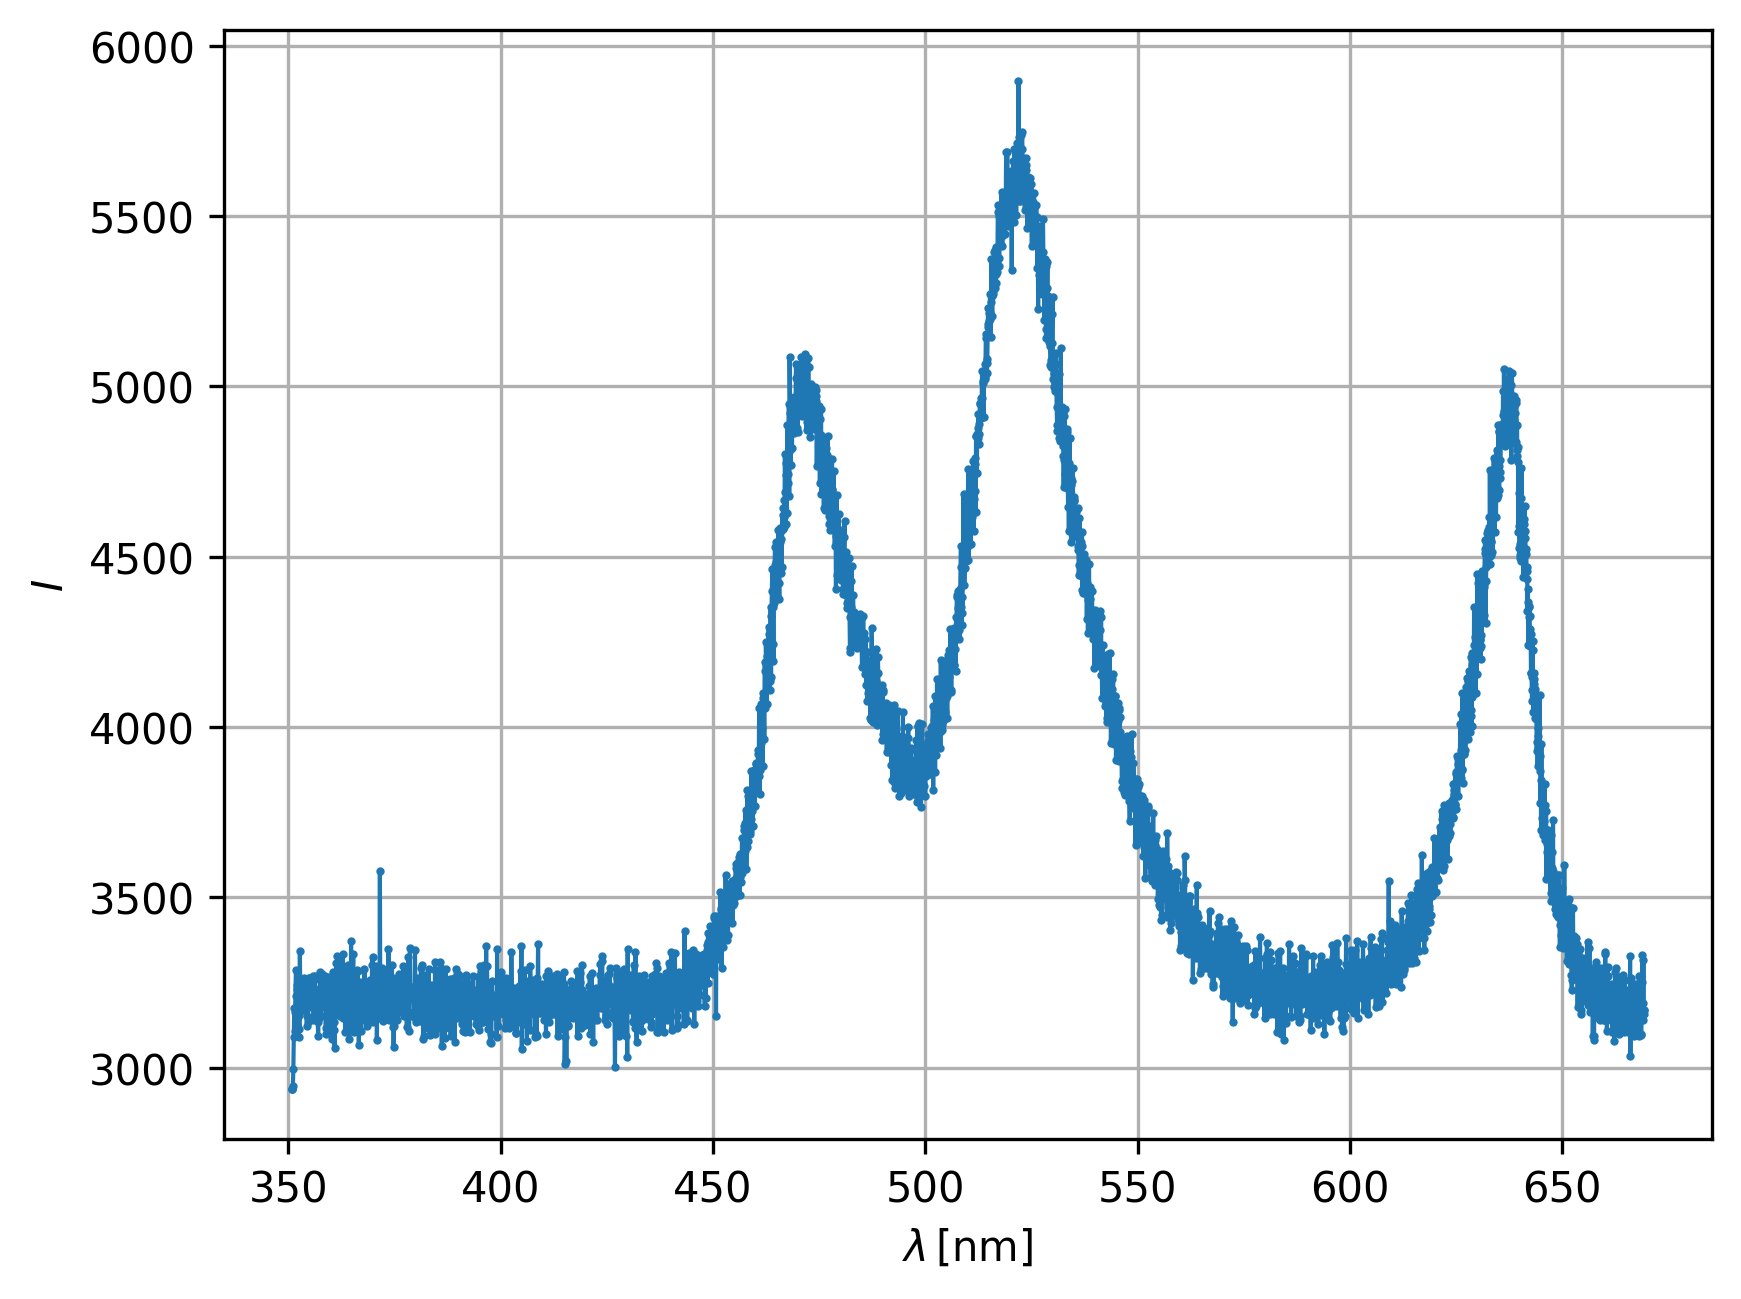
\includegraphics[scale=0.7]{spektrum}
	\caption{Wykres natężenia od długości fali zmierzony przy pomocy spektrometru Flame-T OceanInsight}
	\label{fig:spektrometr}
\end{figure}
Na wykresie widać dokładnie trzy szczyty, które identyfikujemy jako najwyższa wartość w okolicy szczytu. Otrzymaliśmy przy tym wartości:
\[
	\lambda_{\mathrm{blue}} = (472 \pm 6) \, \mathrm{nm}, \quad \lambda_{\mathrm{green}} = (522 \pm 3) \, \mathrm{nm}, \quad \lambda_{\mathrm{red}} = (636 \pm 4) \, \mathrm{nm}
\]
Za błąd uznaliśmy najwększą różnice między długością fali w szczycie i wartościciami zawierającymi się w 95\% intensywności w szczycie.

Następnie przedstawiemy dane uzyskane przez pomiary wykonane przez detektor dla wybudowanego spektrometru (rys~\ref{fig:detektor})
\begin{figure}[H]
	\centering
	\begin{subfigure}{0.45\textwidth}
		\centering
		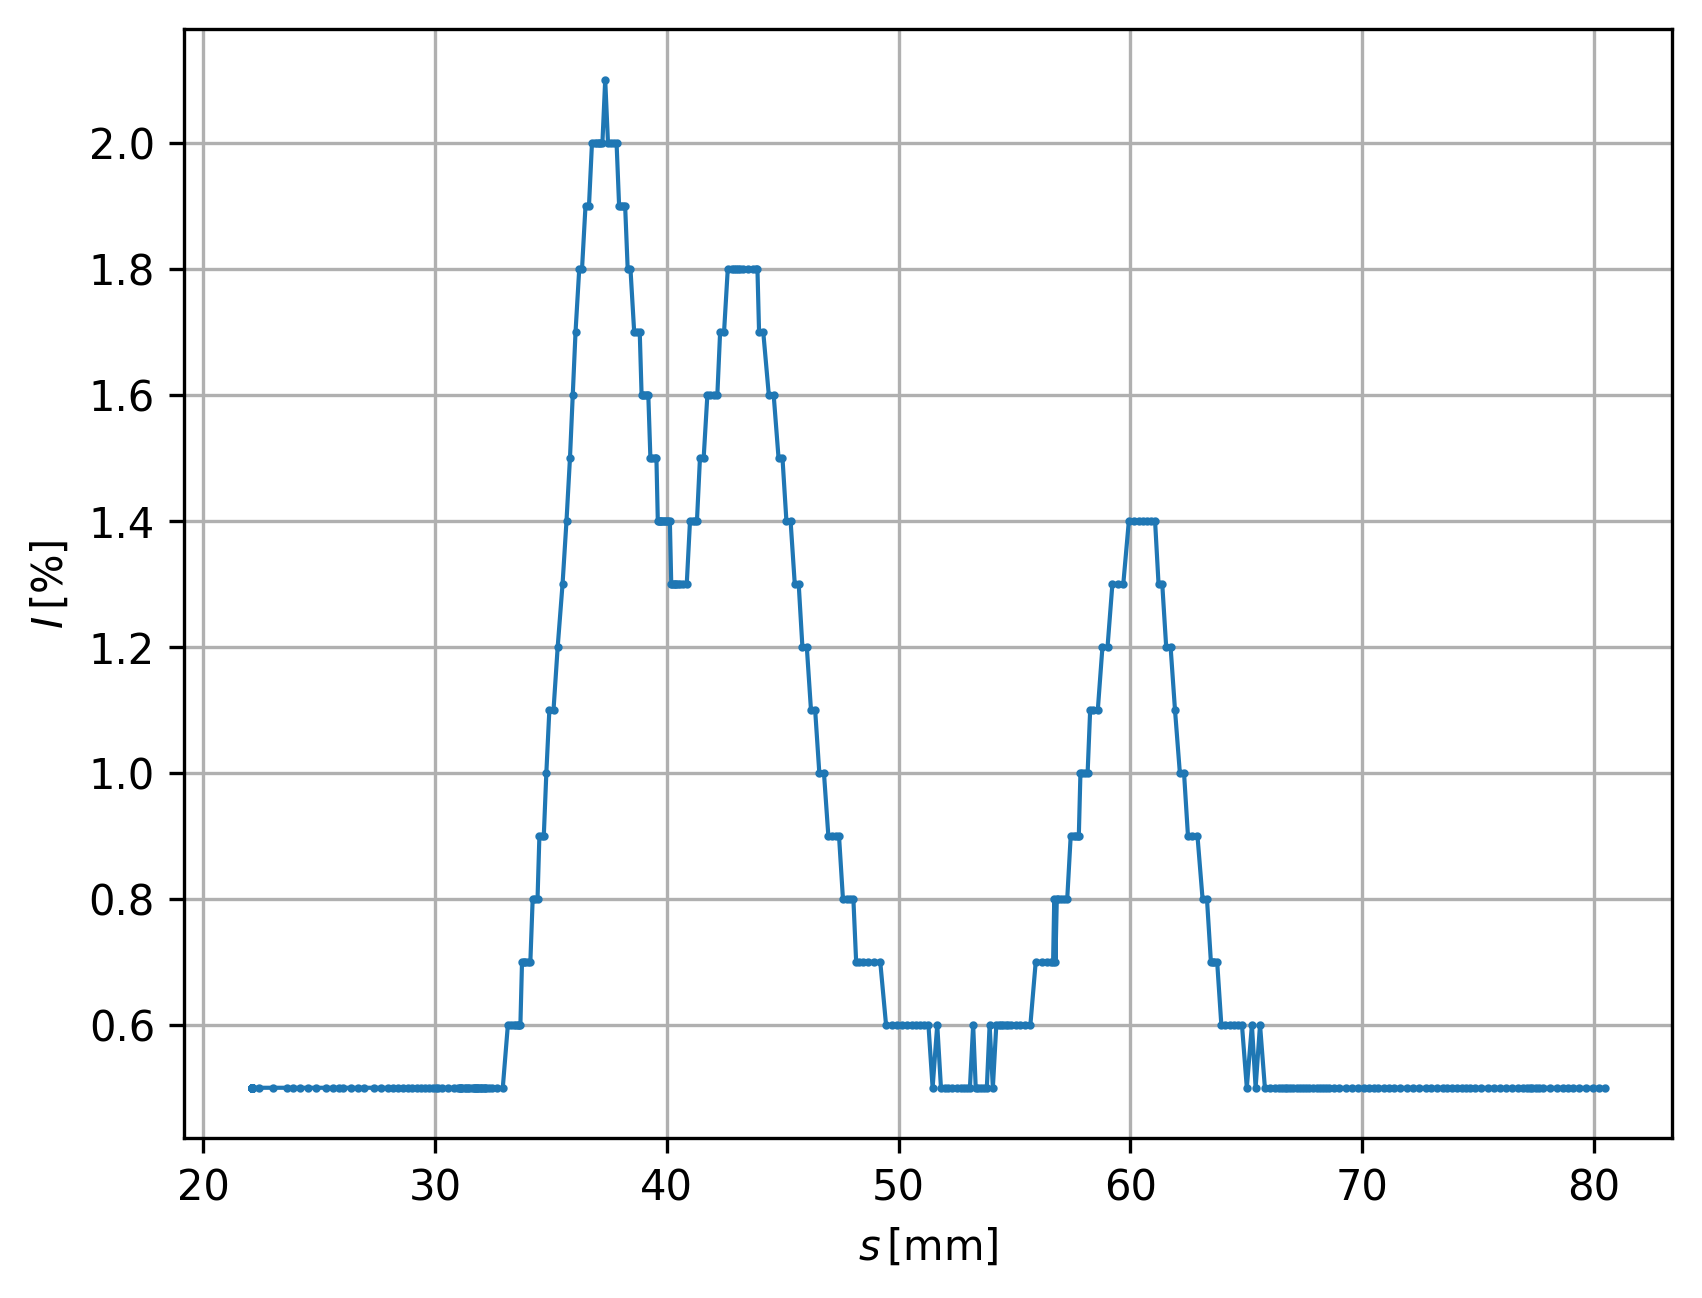
\includegraphics[width=\linewidth]{detektor0}
		\label{fig:detektor_1}
	\end{subfigure}
	\hfill
	\begin{subfigure}{0.45\textwidth}
		\centering
		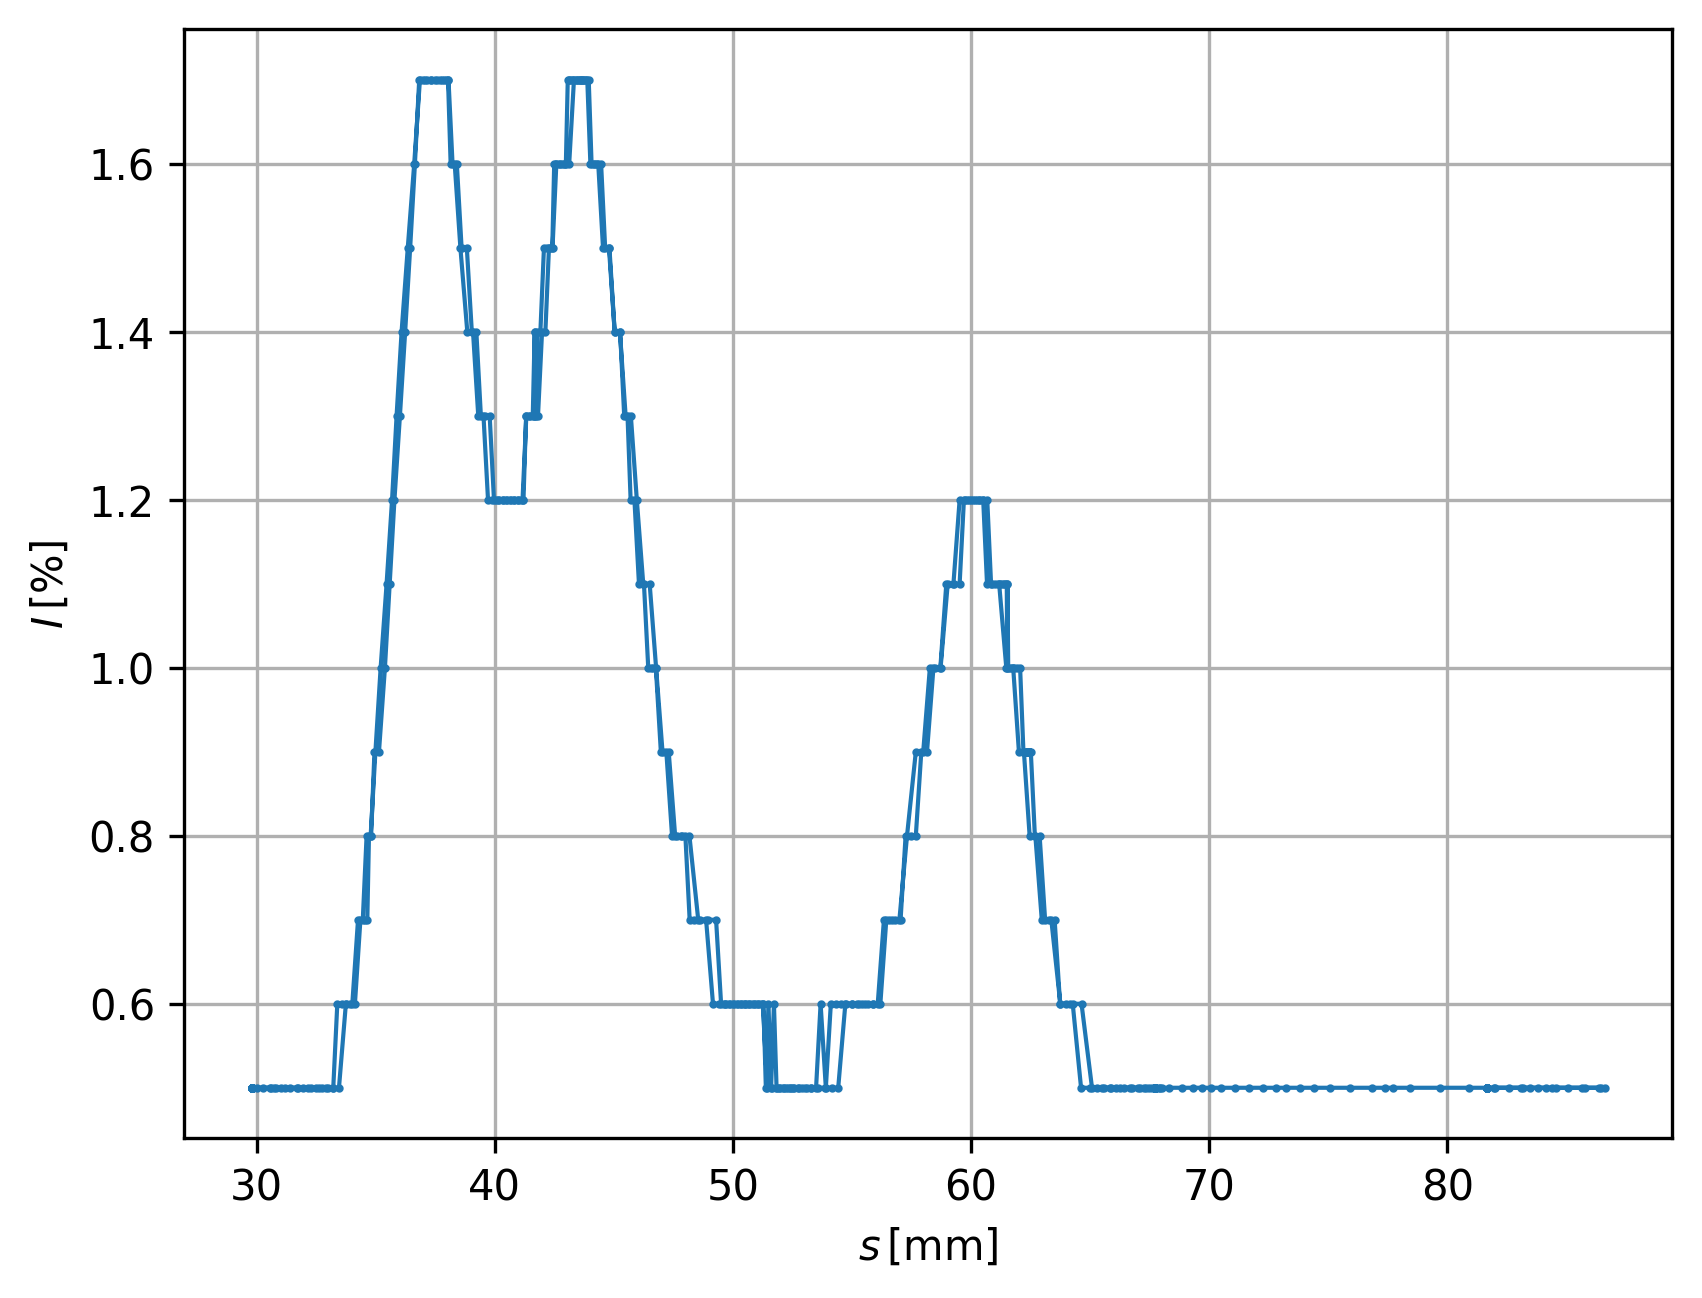
\includegraphics[width=\linewidth]{detektor1}
		\label{fig:detektor_2}
	\end{subfigure}
	\caption{Pomiar natężenia światła od położenia detektora PASCO OS-8441}
	\label{fig:detektor}
\end{figure}
Widzimy że kształt przypomina ten zmierzony spektrometrem komercyjnym. Różnice w intensywności mogą wynikać z absorbcji przyrządów optycznych lub nie idealnym ustawieniu soczewki ustawionej przed detektorem, skupiającej promienie na detektorze.

Dla pierwszego pomiaru (rys.~\ref{fig:detektor_1}) otrzymujemy szczyty intensywności dla:
\[
	y_{\mathrm{blue}} = (37{,}34 \pm 0{,}57) \, \mathrm{nm}, \quad y_{\mathrm{green}} = (42{,}63 \pm 1{,}53) \, \mathrm{nm}, \quad y_{\mathrm{red}} = (59{,}94 \pm 1{,}44) \, \mathrm{nm}
\]
Podczas gdy dla drugiego pomiaru (rys.~\ref{fig:detektor_2}):
\[
	y_{\mathrm{blue}} = (38{,}03 \pm 1{,}21) \, \mathrm{nm}, \quad y_{\mathrm{green}} = (43{,}88 \pm 0{,}82) \, \mathrm{nm}, \quad y_{\mathrm{red}} = (60{,}51 \pm 0{,}99) \, \mathrm{nm}
\]
Błąd otrzymujemy poprzez nawiększą różnice między dystansem w szczycie a tym zawartym w przedziale intensywności 0{,}1 dla pierwszego i 0{,}05 dla drugiego różnicy między maksymalną. Mniejszy błąd dla drugiego wynika z tego że pomiar wykonaliśmy dwukrotnie poruszając detektor w jedną i drugą stronę.

Do tych danych możemy dopasować zależności opisane w \cite{skrypt}. Pierwsza z nich to:
\[
	\lambda = ay + b
\]
Otrzymujemy wykres:
\begin{figure}[H]
	\centering
	\begin{subfigure}{0.45\textwidth}
		\centering
		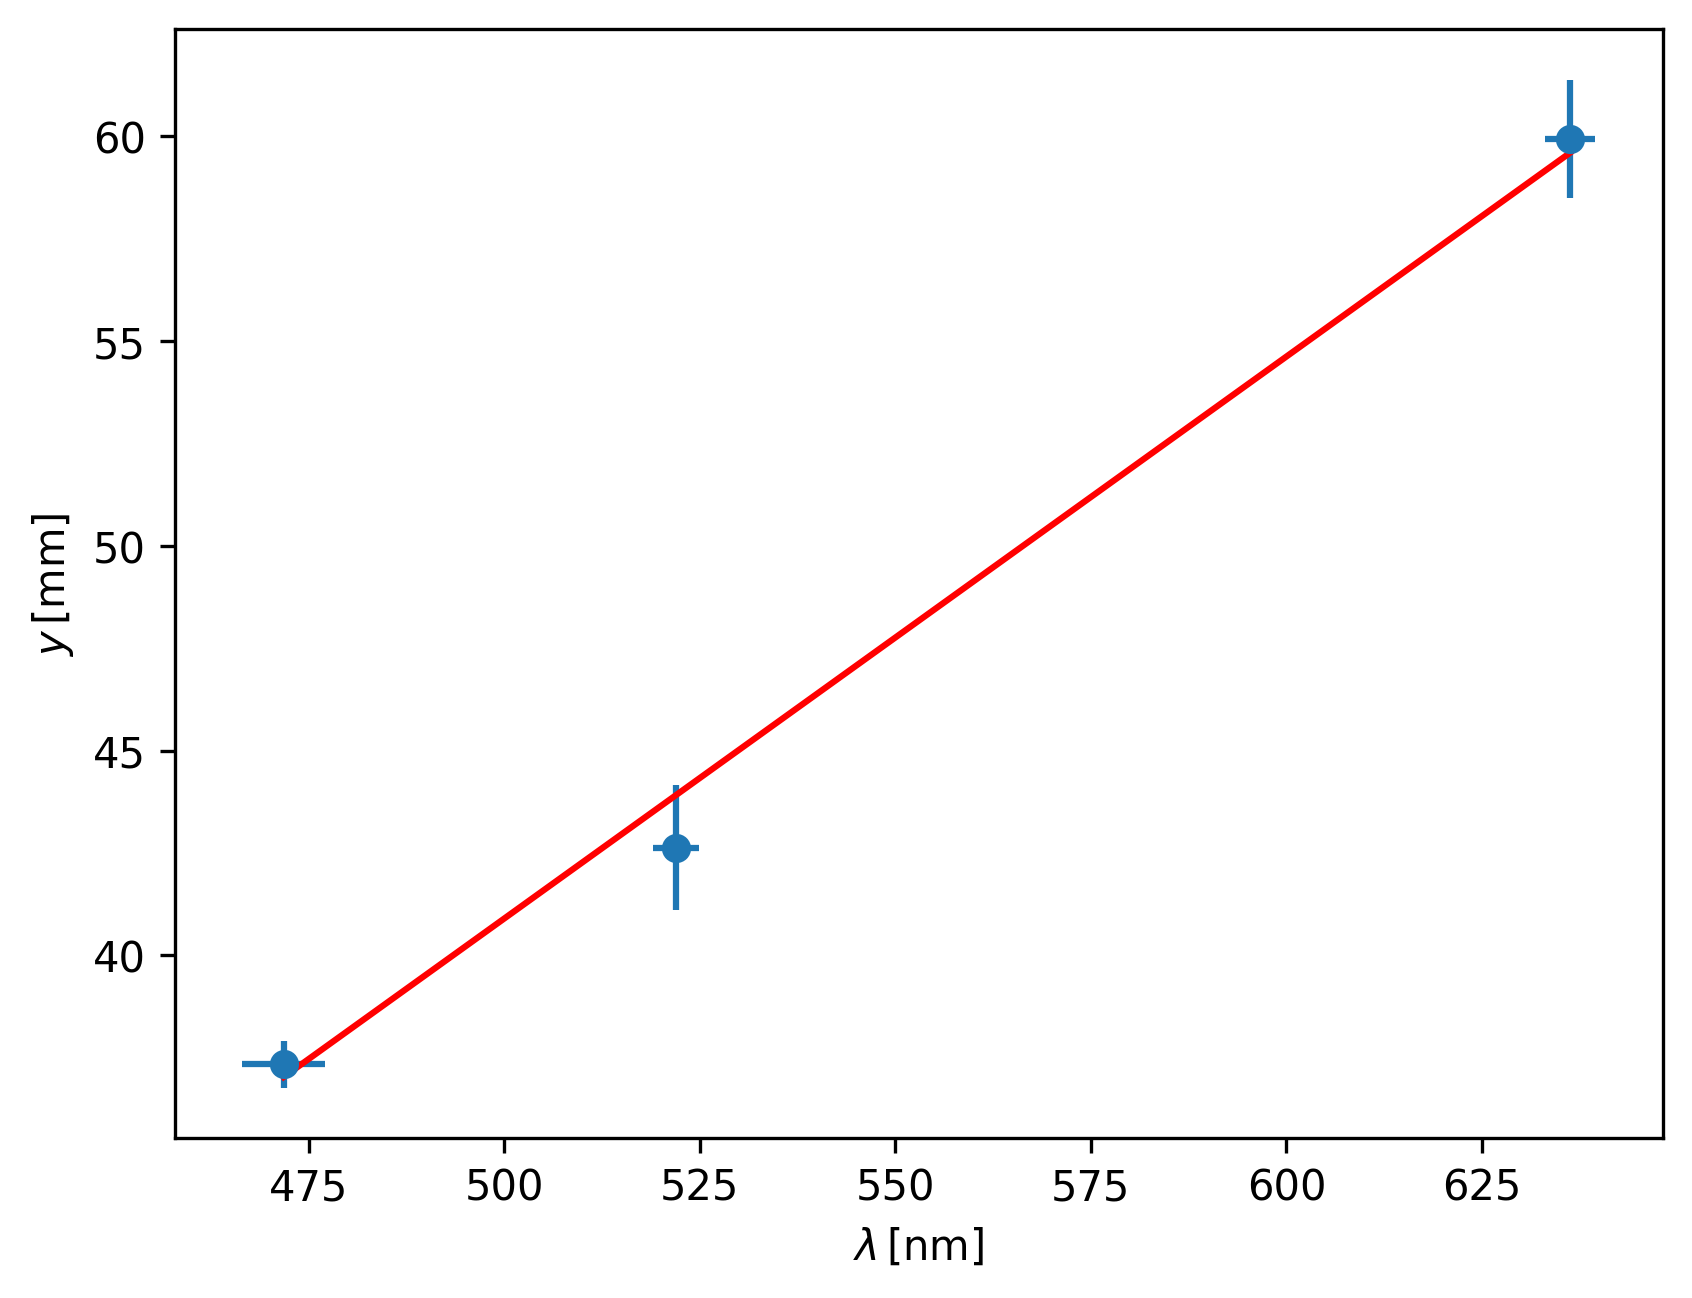
\includegraphics[width=\linewidth]{line_fit_distance_0}
		\label{fig:line_fit_distance_1}
	\end{subfigure}
	\hfill
	\begin{subfigure}{0.45\textwidth}
		\centering
		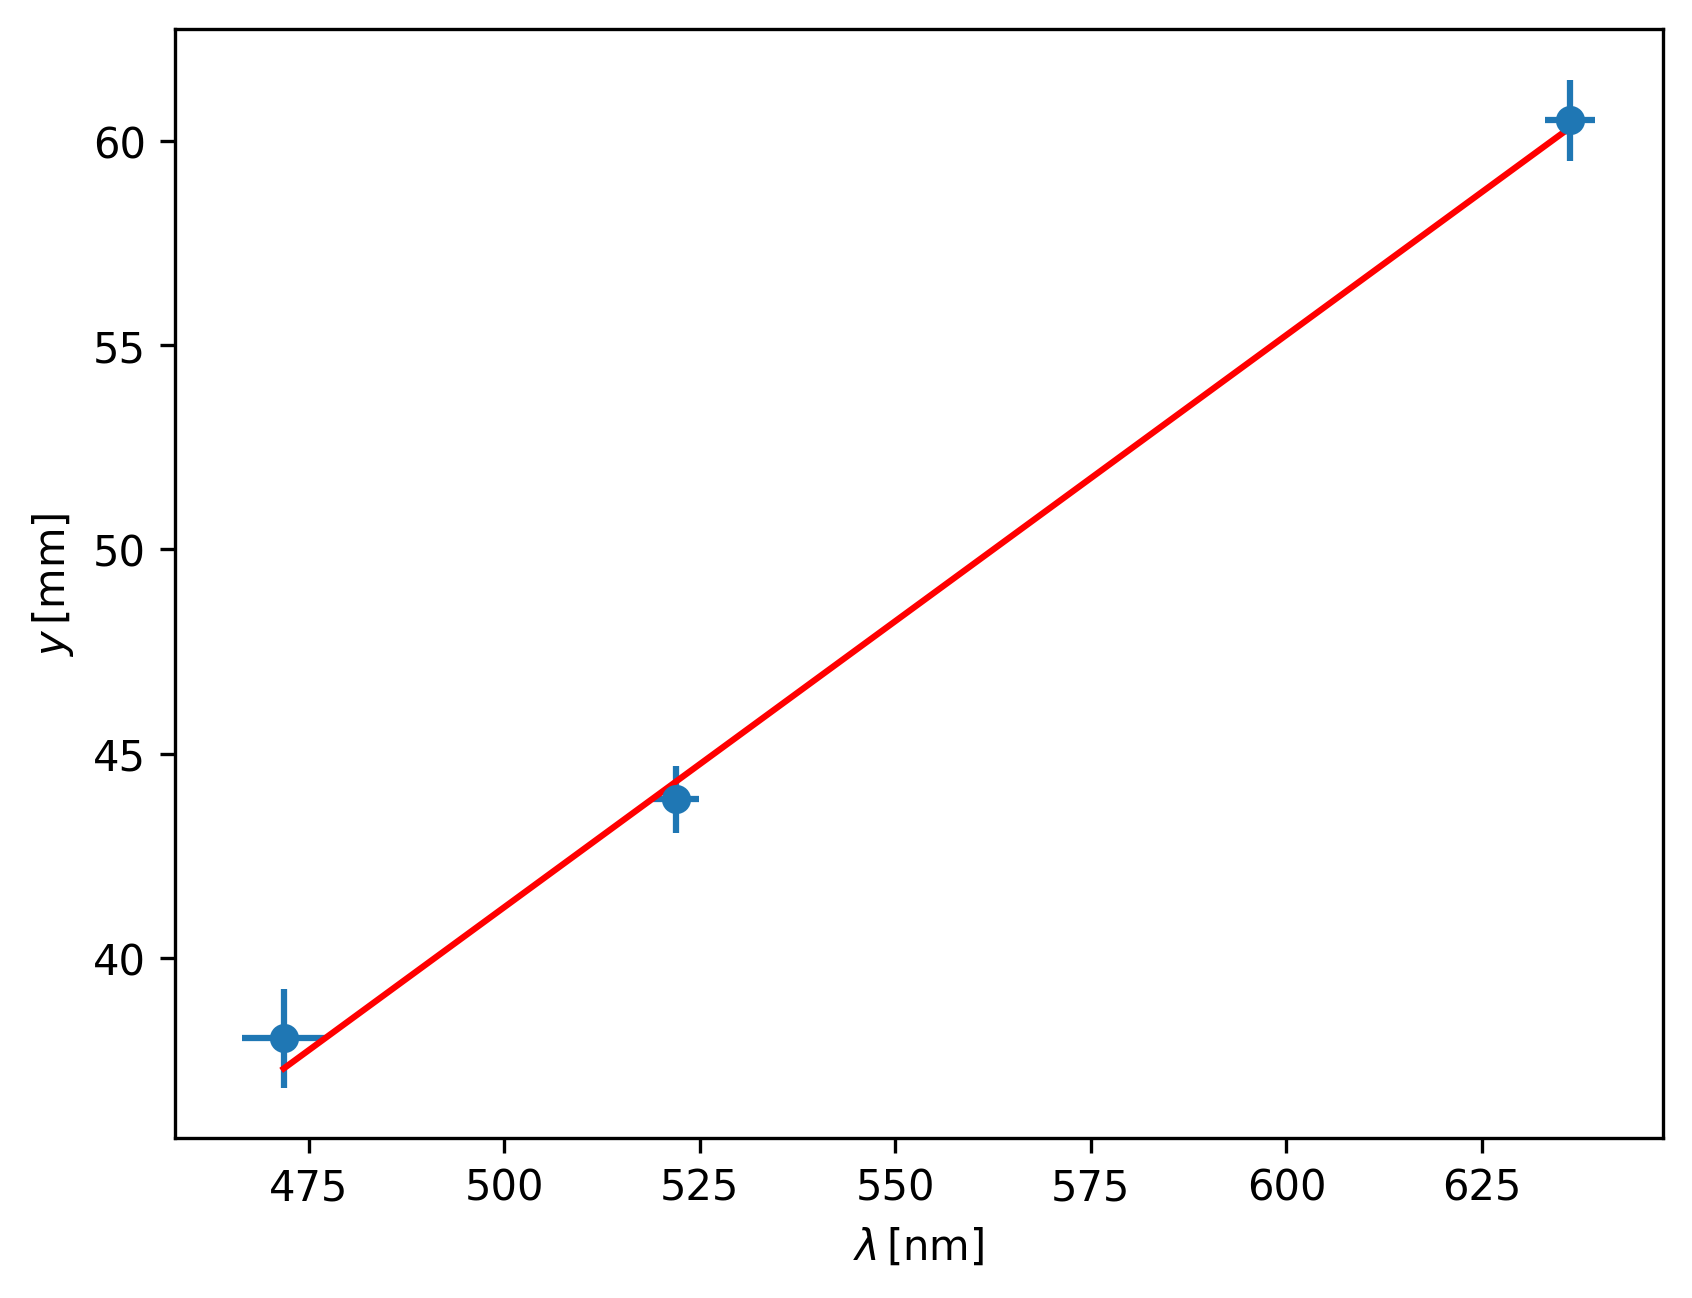
\includegraphics[width=\linewidth]{line_fit_distance_1}
		\label{fig:line_fit_distance_2}
	\end{subfigure}
	\caption{Dopasowanie zależności liniowej do zależności długości fali od położenia}
	\label{fig:line_fit_distance}
\end{figure}
Otrzymujemy przy tym parametry dla pierwszego rysunku~\ref{fig:line_fit_distance_1}:
\[
	a = (0{,}137 \pm 0{,}010) \, \mathrm{\mu m} \quad b = (-28 \pm 6) \, \mathrm{nm}
\]
Wraz z macieżą kowariantną:
\[
	\begin{bmatrix}
		9{,}62237727 \times 10^{-5}  & -4{,}98730063 \times 10^{-2} \\
		-4{,}98730063 \times 10^{-2} & 26{,}2570001
	\end{bmatrix}
\]
A dla drugiej serii (rys.~\ref{fig:line_fit_distance_2}):
\[
	a = (0{,}140 \pm 0{,}008) \, \mathrm{\mu m} \quad b = (-29 \pm 4) \, \mathrm{nm}
\]
covariancja
\[
	\begin{bmatrix}
		5{,}16322078 \times 10^{-5}  & -2{,}84084046 \times 10^{-2} \\
		-2{,}84084046 \times 10^{-2} & 15{,}8387996
	\end{bmatrix}
\]
Wykorzystując średnią warzoną otrzymujemy
\[
	\bar{a} = (0{,}139 \pm 0{,}006) \, \mathrm{\mu m} \quad \bar{b} = (-28 \pm 4) \, \mathrm{nm}
\]
Jeśli jednak chcemy rozważyć drugą zależność opisaną w \cite{skrypt}:
\[
	y = A\lambda + B
\]
Otrzymujemy wtedy wykresy:
\begin{figure}[H]
	\centering
	\begin{subfigure}{0.45\textwidth}
		\centering
		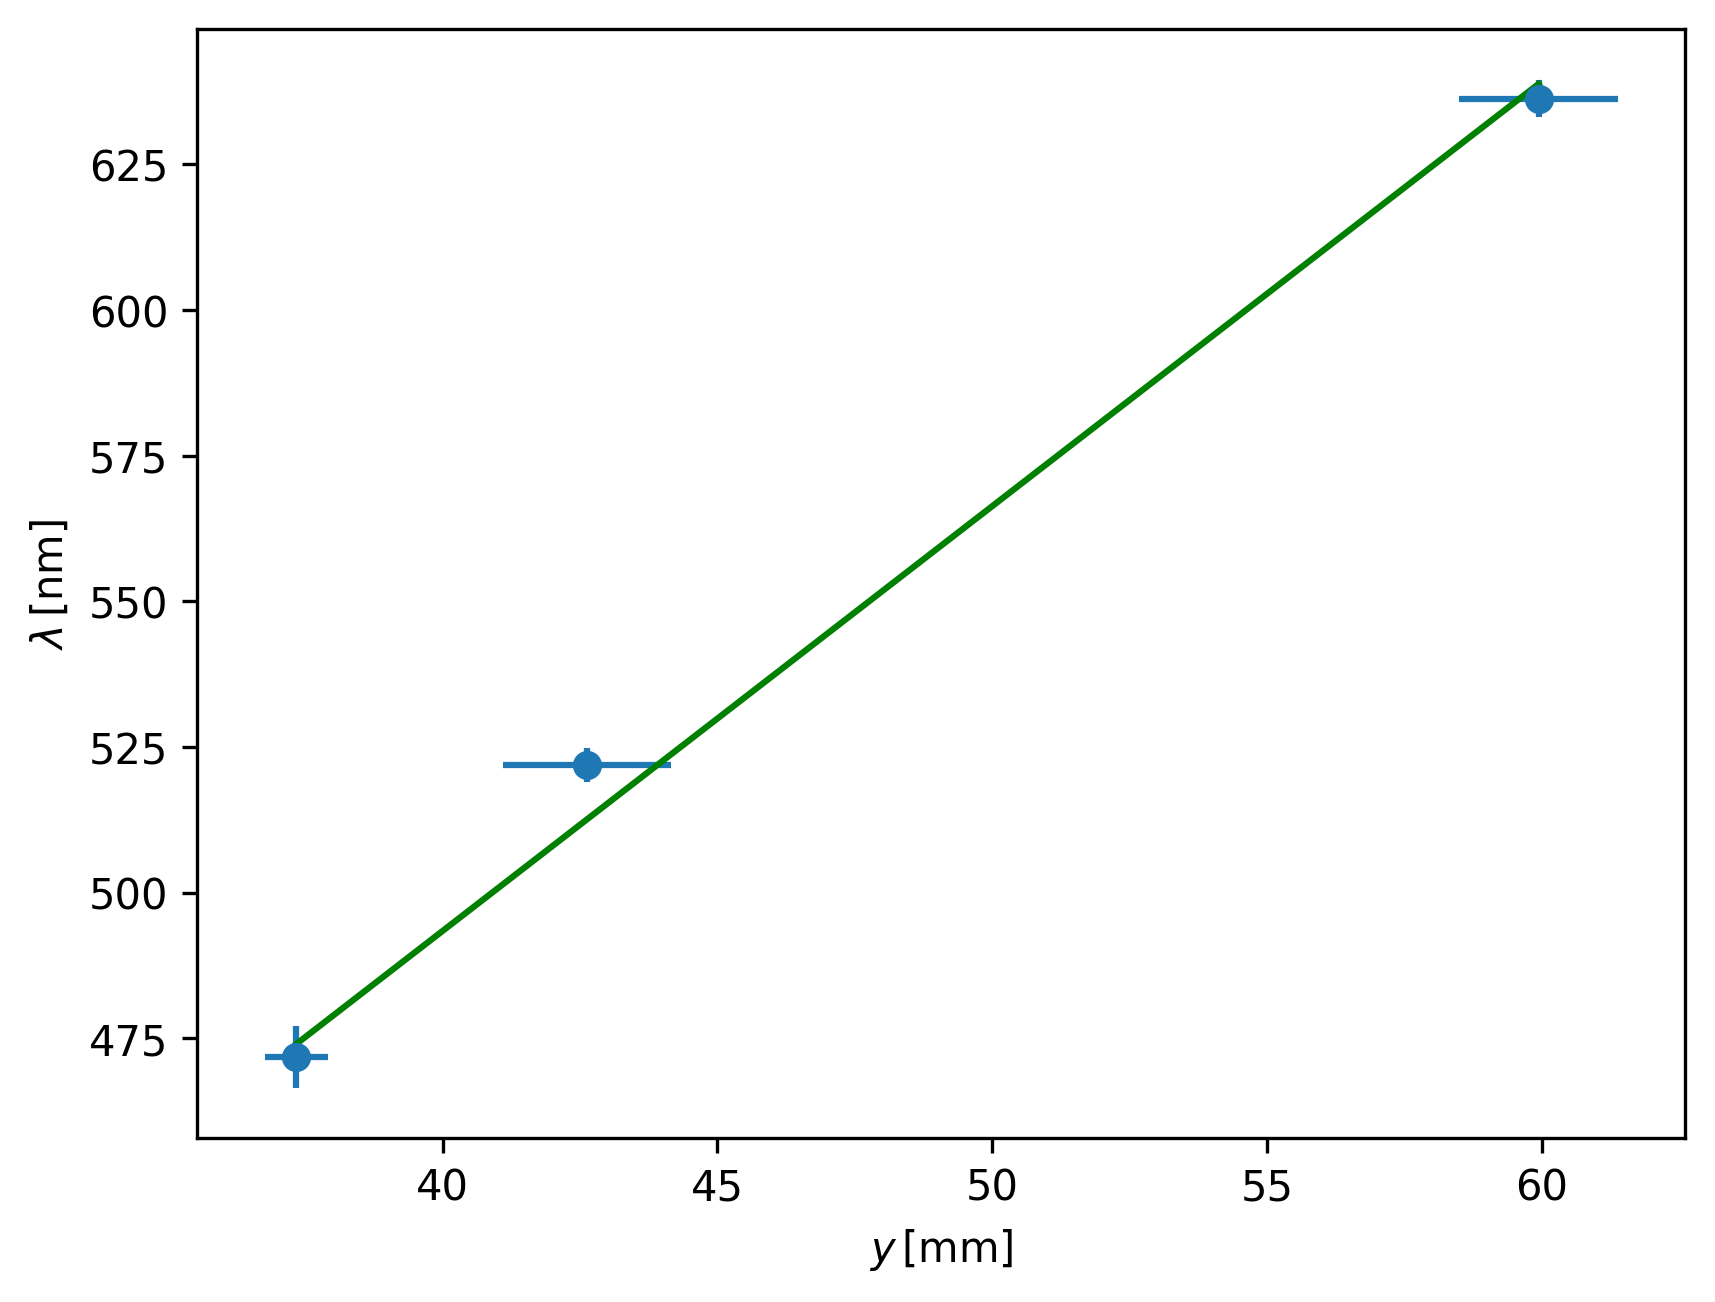
\includegraphics[width=\linewidth]{line_fit_wavelength_0}
		\label{fig:line_fit_wavelength_1}
	\end{subfigure}
	\hfill
	\begin{subfigure}{0.45\textwidth}
		\centering
		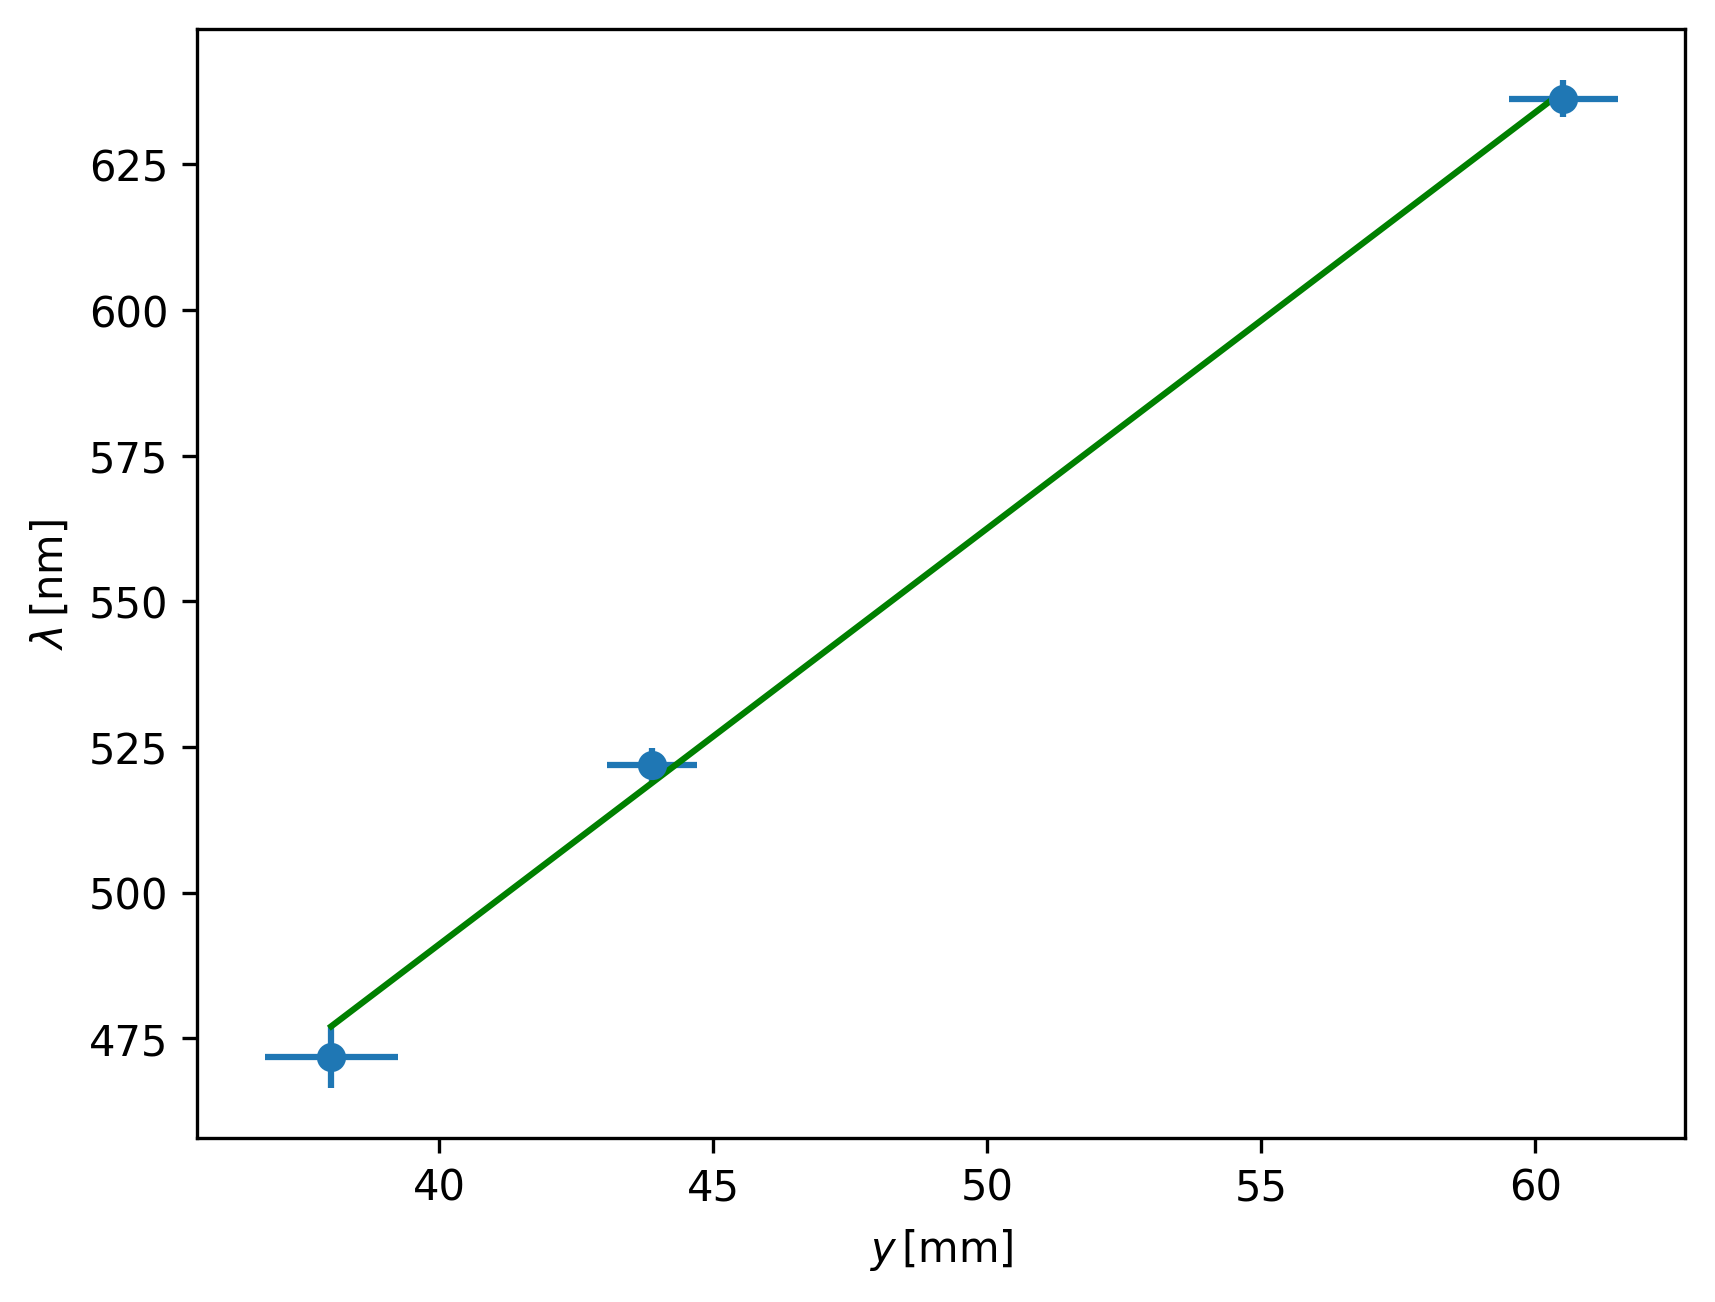
\includegraphics[width=\linewidth]{line_fit_wavelength_1}
		\label{fig:line_fit_wavelength_2}
	\end{subfigure}
	\caption{Dopasowanie zależności liniowej do zależności położenia od długości fali}
	\label{fig:line_fit_wavelength}
\end{figure}
Wtedy pierwszy rysunek~\ref{fig:line_fit_wavelength_1} odpowiada parametrom:
\[
	A = (7{,}29 \pm 0{,}53) \, \mathrm{\mu m} \quad b = (-202 \pm 24) \, \mathrm{nm}
\]
Przy kowariancji
\[
	\begin{bmatrix}
		0{,}271814652 & -11{,}8010188 \\
		-11{,}8010188 & 534{,}018358
	\end{bmatrix}
\]
Podczas gdy dla drugiej serii (rys.~\ref{fig:line_fit_wavelength_2}) otrzymujemy:
\[
	A = (7{,}14 \pm 0{,}37) \, \mathrm{\mu m} \quad b = (-205 \pm 18) \, \mathrm{nm}
\]
Jednocześnie z macieżą kowariantną
\[
	\begin{bmatrix}
		0{,}134202927 & -6{,}47876231 \\
		-6{,}47876231 & 323{,}387243
	\end{bmatrix}
\]
Oraz ponownie korzystając ze średniej ważonej otrzymujemy:
\[
	A = (7{,}19 \pm 0{,}30) \, \mathrm{\mu m} \quad b = (-204 \pm 15) \, \mathrm{nm}
\]
Błędy jakie otrzymaliśmy mogą pochodzić od paru czynników. Przede wszystkim nasz układ był wpierw dopasowywany do lasera, lecz po podmienieniu go na lampe RGB układ trzeba było dostosować aby promienie były dobrze skupione na detektorze, mimo to otrzymane promienie nie były w pełni skupione. Oprócz tego światło docierające do detektora było na tyle nikłe że dokładność detektora zaczeła mieć wpływ na identyfikowanie szczytów. Natomiast niepewność wywołana przez spektroskop przemysłowy jest nikła w porównaniu do wcześniej wspomnianych.
\begin{thebibliography}{1}

	\bibitem{skrypt}
	\emph{Budowa i Kalibracja Spektrometru}, Aneta Drabińska, Uniwersytet Warszawski.

\end{thebibliography}

\end{document}
